\documentclass[aspectratio=169]{beamer}

% ============================================================
% PACKAGES
% ============================================================
\usetheme{Madrid}
\usepackage{cite}
\usepackage[utf8]{inputenc}
\usepackage{graphicx}
\usepackage{tikz}
\usepackage{array}
\usepackage{hyperref}
\usetikzlibrary{positioning,arrows.meta}

% ============================================================
% COLORS
% ============================================================
\definecolor{mainblue}{RGB}{31,78,121}
\definecolor{lightblue}{RGB}{225,238,250}

\setbeamercolor{structure}{fg=mainblue}
\setbeamercolor{frametitle}{fg=white, bg=mainblue}
\setbeamercolor{title}{fg=white, bg=mainblue}

% ============================================================
% FOOTER — TITLE + PAGE NUMBER ONLY
% ============================================================
\setbeamertemplate{footline}{
    \leavevmode%
    \hbox{%
        \begin{beamercolorbox}[
            wd=\paperwidth,
            ht=2.5ex,
            dp=1.2ex,
            leftskip=0.3cm,
            rightskip=0.3cm
        ]{author in head/foot}%
            \insertshorttitle
            \hfill
            \insertframenumber
        \end{beamercolorbox}%
    }
}

\setbeamertemplate{navigation symbols}{}
% ============================================================
% TITLE
% ============================================================
\title[A Graph-Based Semantic-Aware Framework]
{A Graph-Based Semantic-Aware Framework\\
for Vehicular Communications using Veins}

\author{
\textbf{Team Members}\\[0.15cm]
Maisha Sanjida \; (220041128)\\
Mahdi Islam \; (220041149)\\
Saeera Tanjim \; (220041107)
}

\institute{
\textbf{Supervisor:} Md. Mahbub Alam\\
\textbf{Co-Supervisor:} S. M. Sabit Bananee\\
\textbf{Course:} CSE 4610 : Design Project
}

\date{14th September 2026}

\begin{document}

\begin{frame}
    \titlepage
\end{frame}

% ================= Slide 2: Introduction — Vehicular Networks =================
\begin{frame}{Introduction: Vehicular Networks}

\begin{columns}[T,onlytextwidth]

% ---------------- LEFT: TEXT ----------------
\begin{column}{0.58\textwidth}
\begin{itemize}
    \item \textbf{VANETs}: vehicles + roadside units (RSUs) exchange information
    \item \textbf{V2V / V2I} communication for CAVs $\rightarrow$ safer, efficient \textbf{ITS}
    \item Key challenges:
    \begin{itemize}
        \item \textbf{High mobility} $\rightarrow$ dynamic topology
        \item \textbf{Short contact/link duration}
        \item Frequent \textbf{link breakage}, intermittent connectivity
        \item Strict \textbf{latency \& reliability} needs
    \end{itemize}
\end{itemize}
\end{column}

% ---------------- RIGHT: IMAGE PLACEHOLDER ----------------
\begin{column}{0.38\textwidth}
\centering
\includegraphics[width=\linewidth]{figures/ANET-communication-system-is-supported-by-DSRC-which-offers-V2V-and-V2I-communications.png}
\end{column}

\end{columns}

\end{frame}

% ============================================================
% SLIDE — INTRODUCTION: SEMANTIC COMMUNICATION
% ============================================================
\begin{frame}{Introduction: Semantic Communication}

\begin{itemize}
    \item Raw sensor/camera data $\rightarrow$ \textbf{high bandwidth}, hard over unstable links
    \item \textbf{Semantic Communication}: transmit \textbf{meaning}, not raw bits
\end{itemize}

\vspace{0.15cm}

\begin{center}

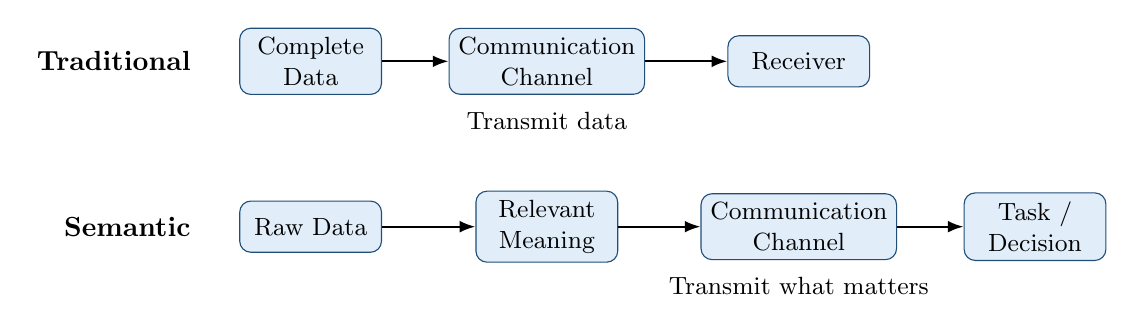
\begin{tikzpicture}[
    box/.style={
        draw=mainblue,
        rounded corners,
        fill=lightblue,
        minimum width=1.8cm,
        minimum height=0.65cm,
        align=center,
        font=\small
    },
    arr/.style={
        -{Latex[length=2mm]},
        thick
    }
]

% ============================================================
% Traditional
% ============================================================

\node[font=\bfseries, anchor=east] at (-5.7,1.0)
{Traditional};

\node[box] (tdata) at (-4.3,1.0)
{Complete\\Data};

\node[box] (tchannel) at (-1.3,1.0)
{Communication\\Channel};

\node[box] (treceiver) at (1.9,1.0)
{Receiver};

\draw[arr] (tdata) -- (tchannel);
\draw[arr] (tchannel) -- (treceiver);

\node[font=\small] at (-1.3,0.25)
{Transmit data};


% ============================================================
% Semantic
% ============================================================

\node[font=\bfseries, anchor=east] at (-5.7,-1.1)
{Semantic};

\node[box] (sdata) at (-4.3,-1.1)
{Raw Data};

\node[box] (smeaning) at (-1.3,-1.1)
{Relevant\\Meaning};

\node[box] (schannel) at (1.9,-1.1)
{Communication\\Channel};

\node[box] (stask) at (4.9,-1.1)
{Task /\\Decision};

\draw[arr] (sdata) -- (smeaning);
\draw[arr] (smeaning) -- (schannel);
\draw[arr] (schannel) -- (stask);

\node[font=\small] at (1.9,-1.85)
{Transmit what matters};

\end{tikzpicture}

\end{center}

\begin{itemize}
    \item[$\Rightarrow$] Lower bandwidth \& latency, task-relevant info preserved
\end{itemize}

\end{frame}


% ============================================================
% SLIDE — SEMANTIC COMMUNICATION: SENDER-RECEIVER PIPELINE
% ============================================================
\begin{frame}{Semantic Communication: Sender–Receiver Pipeline}

\begin{center}

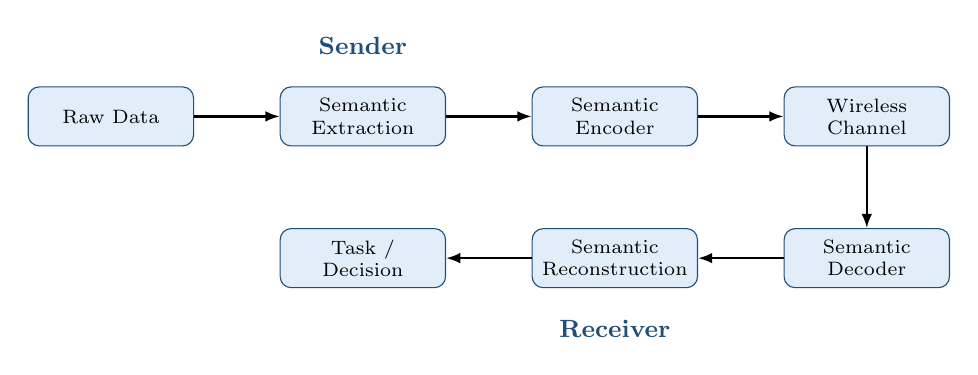
\begin{tikzpicture}[
    box/.style={
        draw=mainblue,
        rounded corners,
        fill=lightblue,
        minimum width=2.1cm,
        minimum height=0.75cm,
        align=center,
        font=\scriptsize
    },
    arr/.style={
        -{Latex[length=1.8mm]},
        thick
    }
]

% ============================================================
% ROW 1 — LEFT TO RIGHT
% ============================================================

\node[box] (raw) at (-4.8,0)
{Raw Data};

\node[box] (extract) at (-1.6,0)
{Semantic\\Extraction};

\node[box] (encode) at (1.6,0)
{Semantic\\Encoder};

\node[box] (channel) at (4.8,0)
{Wireless\\Channel};

\draw[arr] (raw.east) -- (extract.west);
\draw[arr] (extract.east) -- (encode.west);
\draw[arr] (encode.east) -- (channel.west);

\node[font=\small\bfseries, mainblue] at (-1.6,0.9)
{Sender};

% ============================================================
% CONNECT TO ROW 2
% ============================================================

\node[box] (decode) at (4.8,-1.8)
{Semantic\\Decoder};

\node[box] (reconstruct) at (1.6,-1.8)
{Semantic\\Reconstruction};

\node[box] (task) at (-1.6,-1.8)
{Task /\\Decision};

\draw[arr] (channel.south) -- (decode.north);

% ============================================================
% ROW 2 — RIGHT TO LEFT
% ============================================================

\draw[arr] (decode.west) -- (reconstruct.east);
\draw[arr] (reconstruct.west) -- (task.east);

\node[font=\small\bfseries, mainblue] at (1.6,-2.7)
{Receiver};

\end{tikzpicture}

\end{center}

\vspace{0.15cm}

\begin{itemize}
    \item \textbf{Sender}: extract + encode task-relevant information
    \item Only \textbf{semantic info} crosses the wireless channel
    \item \textbf{Receiver}: decode + reconstruct for the task
    \item Evaluated in \textbf{Veins} (vehicular network simulation)
\end{itemize}

\end{frame}
% ============================================================
% SLIDE — WHY SEMANTIC COMMUNICATION FOR CAVs?
% ============================================================
\begin{frame}{Why Semantic Communication for CAVs?}

\centering

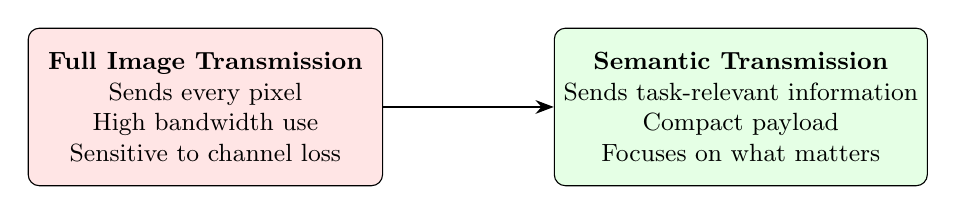
\begin{tikzpicture}[
    box/.style={
        rectangle,
        draw,
        rounded corners,
        minimum width=4.5cm,
        minimum height=2.0cm,
        align=center,
        font=\small
    },
    arrow/.style={
        -Stealth,
        thick
    }
]

\node[box, fill=red!10] (full) at (0,0)
{\textbf{Full Image Transmission}\\
Sends every pixel\\
High bandwidth use\\
Sensitive to channel loss};

\node[box, fill=green!10] (sem) at (6.8,0)
{\textbf{Semantic Transmission}\\
Sends task-relevant information\\
Compact payload\\
Focuses on what matters};

\draw[arrow] (full) -- node[above, font=\footnotesize]
{} (sem);

\end{tikzpicture}

\vspace{0.45cm}


\begin{center}


\vspace{0.1cm}

CAVs exchange large amounts of road-scene data over wireless networks.

Semantic communication can reduce this burden by transmitting only
\textbf{task-relevant information}.
\end{center}

\end{frame}

% ============================================================
% SLIDE 5 — MOTIVATION
% ============================================================
\begin{frame}{Motivation}

\begin{center}

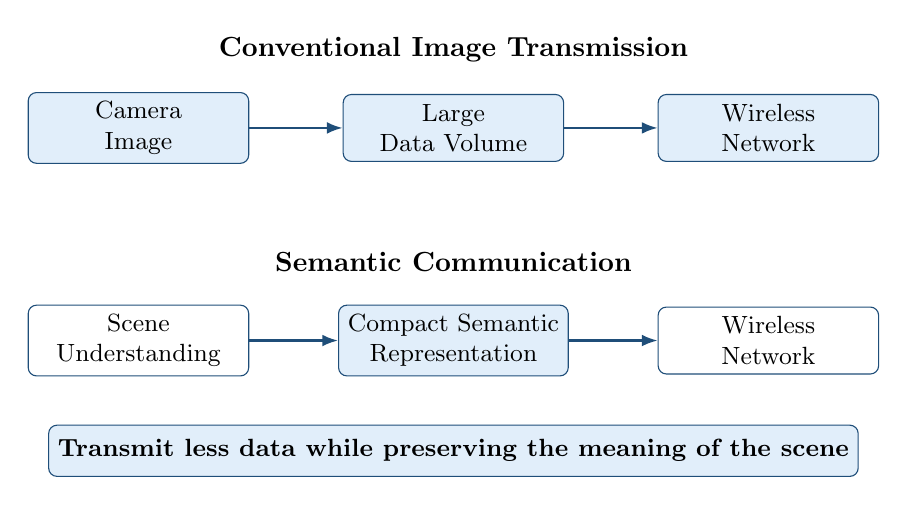
\begin{tikzpicture}[
    box/.style={
        draw=mainblue,
        rounded corners=3pt,
        fill=lightblue,
        minimum width=2.8cm,
        minimum height=0.85cm,
        align=center,
        font=\small
    },
    smallbox/.style={
        draw=mainblue,
        rounded corners=3pt,
        fill=white,
        minimum width=2.8cm,
        minimum height=0.85cm,
        align=center,
        font=\small
    },
    arr/.style={
        -{Latex[length=2mm]},
        thick,
        mainblue
    }
]

% ---------------- Conventional approach ----------------
\node[font=\normalsize\bfseries] at (0,0) {Conventional Image Transmission};

\node[box] (camera1) at (-4,-1) {Camera\\Image};
\node[box] (data1) at (0,-1) {Large\\Data Volume};
\node[box] (network1) at (4,-1) {Wireless\\Network};

\draw[arr] (camera1) -- (data1);
\draw[arr] (data1) -- (network1);

% ---------------- Semantic approach ----------------
\node[font=\normalsize\bfseries] at (0,-2.7) {Semantic Communication};

\node[smallbox] (camera2) at (-4,-3.7) {Scene\\Understanding};
\node[box] (data2) at (0,-3.7) {Compact Semantic\\Representation};
\node[smallbox] (network2) at (4,-3.7) {Wireless\\Network};

\draw[arr] (camera2) -- (data2);
\draw[arr] (data2) -- (network2);

% ---------------- Goal ----------------
\node[
    draw=mainblue,
    rounded corners=3pt,
    fill=lightblue,
    minimum width=9cm,
    minimum height=0.65cm,
    align=center,
    font=\small\bfseries
] at (0,-5.1)
{Transmit less data while preserving the meaning of the scene};

\end{tikzpicture}

\end{center}

\end{frame}


% ============================================================
% SLIDE — RELATED WORK
% ============================================================
\begin{frame}{Key Related Work}

\begin{itemize}

    \item \textbf{Scene-Graph Augmented Risk Assessment \cite{yu2020scene}}
    \begin{itemize}
        \item Represents driving scenes as graphs of objects and relationships.
        \item Uses GNN/LSTM models for driving risk assessment.
        \item Establishes structured scene representation for autonomous driving.
    \end{itemize}

    \vspace{0.12cm}

    \item \textbf{SEECAD: Semantic Communication for CAVs \cite{ribouh2024seecad}}
    \begin{itemize}
        \item Transmits semantic information instead of raw image pixels.
        \item Uses MobileNetV2 with LDPC coding and QAM modulation.
        \item Shows semantic communication can reduce transmission requirements.
    \end{itemize}

    \vspace{0.12cm}

    \item \textbf{Knowledge Graph Representation Learning
    \cite{hello2024knowledge}}
    \begin{itemize}
        \item Represents knowledge using compact graph embeddings.
        \item Reconstructs graph relations at the receiver.
        \item Enables communication-efficient graph transmission.
    \end{itemize}

\end{itemize}

\end{frame}


% ============================================================
% SLIDE — GBSED
% ============================================================
\begin{frame}{GBSED: From Semantic Representation to Risk Assessment}

\begin{itemize}

    \item \textbf{GBSED (Graph Based Semantic Encoder Decoder) \cite{ribouh2026gbsed}}
    \begin{itemize}
        \item Encodes driving scene graphs into a compact tensor
        representation for semantic transmission.
        \item Applies relation-based semantic compression to remove
        redundant graph information.
        \item Reconstructs the task-relevant scene graph and uses a
        \textbf{GNN + LSTM + MLP} for downstream risk assessment.
    \end{itemize}

    \vspace{0.15cm}

    \item \textbf{Reported performance}
    \begin{itemize}
        \item Approximately \textbf{99.9\% data reduction}.
        \item Semantic fidelity above \textbf{0.9} at SNR $>10$ dB.
    \end{itemize}

    \vspace{0.15cm}

    \item \textbf{Evaluation}
    \begin{itemize}
        \item MIMO-OFDM channel with 3GPP CDL using \textbf{Sionna}.
        \item Focuses on physical-layer semantic transmission rather than
        full network-level vehicular communication.
    \end{itemize}

\end{itemize}

\end{frame}

% ==============================================================
% SLIDE 7 — GBSED
% ============================================================
\begin{frame}{GBSED: Graph-Based Semantic Communication}

\begin{center}

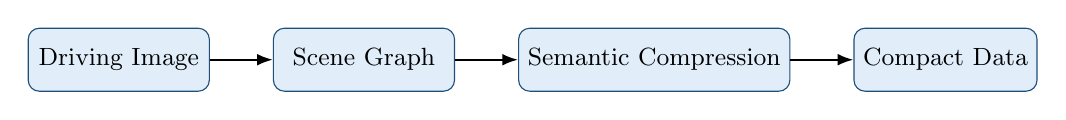
\begin{tikzpicture}[
    box/.style={
        draw=mainblue,
        rounded corners,
        fill=lightblue,
        minimum width=2.3cm,
        minimum height=0.8cm,
        align=center,
        font=\small
    },
    arr/.style={
        -{Latex[length=2mm]},
        thick
    }
]

\node[box] (image) {Driving Image};
\node[box, right=0.8cm of image] (graph) {Scene Graph};
\node[box, right=0.8cm of graph] (compress) {Semantic Compression};
\node[box, right=0.8cm of compress] (data) {Compact Data};

\draw[arr] (image) -- (graph);
\draw[arr] (graph) -- (compress);
\draw[arr] (compress) -- (data);

\end{tikzpicture}

\vspace{0.4cm}

\small\textbf{Scene Graph}

\vspace{0.15cm}

\begin{itemize}
    \item Represents the road scene using \textbf{objects and their relationships}.
    \item \textbf{Nodes:} Vehicles, pedestrians, lanes, etc.
    \item \textbf{Relations:} Relative position and interactions between objects.
    \item \textbf{Features:} Relevant information describing each object.
\end{itemize}

\vspace{0.2cm}

{\small
\textit{The scene is converted from raw visual data into a structured,
task-relevant representation.}
}

\end{center}

\end{frame}

% ============================================================
% SLIDE 8 — GBSED SUMMARY
% ============================================================
\begin{frame}{GBSED:How it works}

\begin{center}

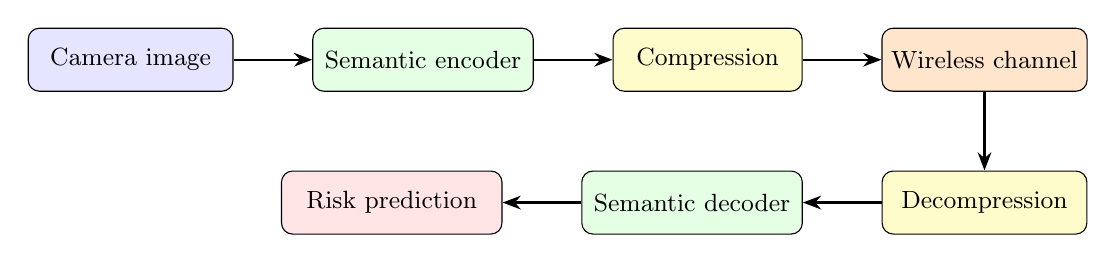
\begin{tikzpicture}[
node distance=1.0cm,
>=Stealth,
every node/.style={font=\small}
]

\node[draw, rounded corners, fill=blue!10,
minimum width=2.6cm,
minimum height=0.8cm] (cam)
{Camera image};

\node[draw, rounded corners, fill=green!10,
right=of cam,
minimum width=2.8cm,
minimum height=0.8cm] (enc)
{Semantic encoder};

\node[draw, rounded corners, fill=yellow!20,
right=of enc,
minimum width=2.4cm,
minimum height=0.8cm] (comp)
{Compression};

\node[draw, rounded corners, fill=orange!20,
right=of comp,
minimum width=2.6cm,
minimum height=0.8cm] (chan)
{Wireless channel};

\node[draw, rounded corners, fill=yellow!20,
below=of chan,
minimum width=2.6cm,
minimum height=0.8cm] (decomp)
{Decompression};

\node[draw, rounded corners, fill=green!10,
left=of decomp,
minimum width=2.8cm,
minimum height=0.8cm] (dec)
{Semantic decoder};

\node[draw, rounded corners, fill=red!10,
left=of dec,
minimum width=2.8cm,
minimum height=0.8cm] (task)
{Risk prediction};

\draw[->, thick] (cam) -- (enc);
\draw[->, thick] (enc) -- (comp);
\draw[->, thick] (comp) -- (chan);
\draw[->, thick] (chan) -- (decomp);
\draw[->, thick] (decomp) -- (dec);
\draw[->, thick] (dec) -- (task);

\end{tikzpicture}

\end{center}

\vspace{0.5cm}

{\small
\textbf{Our Approach:} Built an end-to-end pipeline integrating
\textbf{GBSED semantic processing with Veins/OMNeT++} for vehicular communication evaluation.
}

\end{frame}


% ============================================================
% SLIDE 11 — METHODOLOGY (OVERVIEW)
% ============================================================
\begin{frame}{Methodology: Overview}

\begin{center}
\resizebox{\textwidth}{!}{%
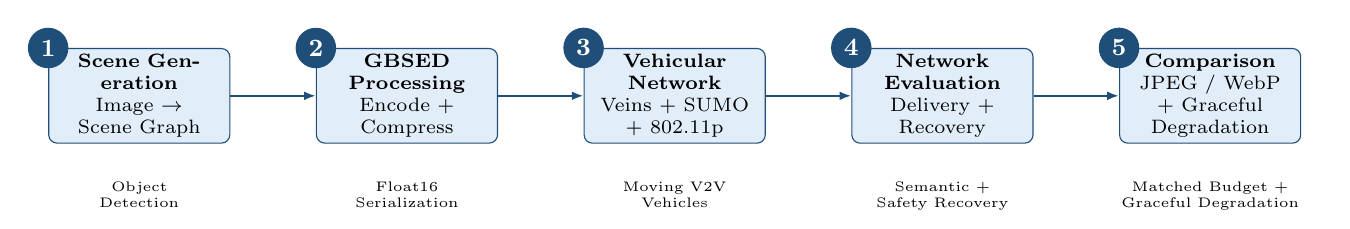
\begin{tikzpicture}[
    box/.style={
        draw=mainblue,
        rounded corners=3pt,
        fill=lightblue,
        minimum width=2.3cm,
        minimum height=1cm,
        text width=2.1cm,
        align=center,
        font=\scriptsize,
        inner sep=2pt
    },
    lbl/.style={
        align=center,
        font=\tiny,
        text width=2.6cm,
        text depth=0pt
    },
    num/.style={
        circle,
        draw=mainblue,
        fill=mainblue,
        text=white,
        font=\bfseries\small,
        inner sep=1pt,
        minimum size=5mm
    },
    arr/.style={
        -{Latex[length=1.5mm]},
        thick,
        mainblue
    }
]

% ============================================================
% MAIN WORKFLOW — LEFT TO RIGHT
% ============================================================

\node[box] (scene) at (0,0)
{\textbf{Scene Generation}\\
Image $\rightarrow$ Scene Graph};

\node[box] (gbsed) at (3.4,0)
{\textbf{GBSED Processing}\\
Encode + Compress};

\node[box] (network) at (6.8,0)
{\textbf{Vehicular Network}\\
Veins + SUMO + 802.11p};

\node[box] (eval) at (10.2,0)
{\textbf{Network Evaluation}\\
Delivery + Recovery};

\node[box] (compare) at (13.6,0)
{\textbf{Comparison}\\
JPEG / WebP + Graceful Degradation};

% Arrows
\draw[arr] (scene.east) -- (gbsed.west);
\draw[arr] (gbsed.east) -- (network.west);
\draw[arr] (network.east) -- (eval.west);
\draw[arr] (eval.east) -- (compare.west);

% Stage numbers (anchor the next slide's grouping to these)
\node[num] at (scene.north west) {1};
\node[num] at (gbsed.north west) {2};
\node[num] at (network.north west) {3};
\node[num] at (eval.north west) {4};
\node[num] at (compare.north west) {5};

% ============================================================
% DETAILS — manual line breaks, no auto-wrap surprises
% ============================================================

\node[lbl] at (0,-1.15) {Object\\Detection};
\node[lbl] at (3.4,-1.15) {Float16\\Serialization};
\node[lbl] at (6.8,-1.15) {Moving V2V\\Vehicles};
\node[lbl] at (10.2,-1.15) {Semantic +\\Safety Recovery};
\node[lbl] at (13.6,-1.15) {Matched Budget +\\Graceful Degradation};

\end{tikzpicture}%
}
\end{center}

\vspace{0.35cm}

\begin{itemize}

    \item \textbf{Semantic pipeline (1–2):}
    convert road images into compact GBSED scene-graph payloads.

    \item \textbf{Network experiments (3–4):}
    transmit payloads between moving vehicles under different channel conditions.

    \item \textbf{Evaluation (5):}
    compare GBSED with JPEG/WebP at matched byte budgets and test
    graceful degradation of the semantic payload.

\end{itemize}

\end{frame}


% % ============================================================
% % SLIDE 12 — METHODOLOGY (PROCESSING STAGES, MAPPED TO OVERVIEW)
% % ============================================================
% \begin{frame}{Methodology: Processing Stages}

% \begin{enumerate}

%     \item[\textbf{1}] \textbf{Scene Understanding}

%     Road image $\rightarrow$ Scene graph

%     \item[\textbf{2}] \textbf{GBSED Processing}

%     \begin{enumerate}
%         \item \textbf{Semantic Representation:}
%         Scene graph $\rightarrow \left(T,\;F\right)$

%         \scriptsize
%         $T$: relation tensor, $F$: node features
%         \normalsize

%         \item \textbf{Semantic Compression:}
%         Remove relation types absent from the scene

%         \item \textbf{Serialization:}
%         Compressed representation $\rightarrow$ Float16 bytes
%     \end{enumerate}

%     \item[\textbf{3}] \textbf{Vehicular Network Transmission}

%     Bytes $\rightarrow$ chunks $\rightarrow$ Base64 $\rightarrow$
%     IEEE 802.11p

%     \item[\textbf{4}] \textbf{Network Evaluation / Reconstruction}

%     Received bytes $\rightarrow$ deserialization $\rightarrow$
%     semantic decompression $\rightarrow$ scene graph

% \end{enumerate}

% \vspace{0.2cm}
% \textit{\footnotesize Stage 5 (Comparison against JPEG/WebP) is covered
% in the evaluation section.}

% \end{frame}



% ============================================================
% SLIDE 11 — IMPLEMENTATION
% ============================================================
\begin{frame}{Implementation: What We Did}

\begin{columns}[T]

\column{0.48\textwidth}

\textbf{Semantic Layer}

\begin{itemize}
    \item Consolidated GBSED processing
    \item Integrated RoadScene2Vec
    \item CPU-compatible Faster R-CNN
    \item Unified serialization / deserialization
    \item Encode--decode validation
\end{itemize}

\column{0.48\textwidth}

\textbf{Network \& Evaluation}

\begin{itemize}
    \item GBSED--Veins integration
    \item Binary payload generation
    \item Moving SUMO vehicles
    \item IEEE 802.11p transmission
    \item Per-chunk TX/RX logging
    \item JPEG / WebP baselines
\end{itemize}

\end{columns}

\vspace{0.25cm}

\begin{center}
\textit{The published GBSED model was used as the semantic foundation;
no GBSED retraining was performed.}
\end{center}

\end{frame}

% ============================================================
% SLIDE 12 — OUR CONTRIBUTION
% ============================================================
\begin{frame}{Our Contribution}

\begin{columns}[T]

\column{0.48\textwidth}

\textbf{What We Built}

\begin{itemize}
    \item Integrated \textbf{GBSED with Veins}
    \item Connected \textbf{GBSED--OMNeT++--SUMO}
    \item Implemented binary payload transmission from extracted scene graph
    \item Enabled semantic graph reconstruction
\end{itemize}

\column{0.48\textwidth}

\textbf{What We Evaluated}

\begin{itemize}
    \item Semantic delivery over \textbf{802.11p}
    \item Packet delivery under different channel conditions
    \item \textbf{GBSED vs JPEG / WebP} at matched budgets
    \item Semantic recovery and safety relations
    \item \textbf{Graceful degradation} using GBSED
\end{itemize}

\end{columns}

\vspace{0.3cm}

\begin{center}
\setlength{\fboxsep}{8pt}
\fcolorbox{mainblue}{lightblue}{
\begin{minipage}{0.82\textwidth}
\centering
\textbf{Main Contribution:}\\
Extending GBSED from a physical-layer semantic communication model
to a \textbf{network-level vehicular communication evaluation}
using Veins, SUMO, and IEEE 802.11p.
\end{minipage}
}
\end{center}

\end{frame}
% ============================================================
% SLIDE 12 — ARCHITECTURE
% ============================================================
\begin{frame}{Implementation Architecture}

\begin{center}

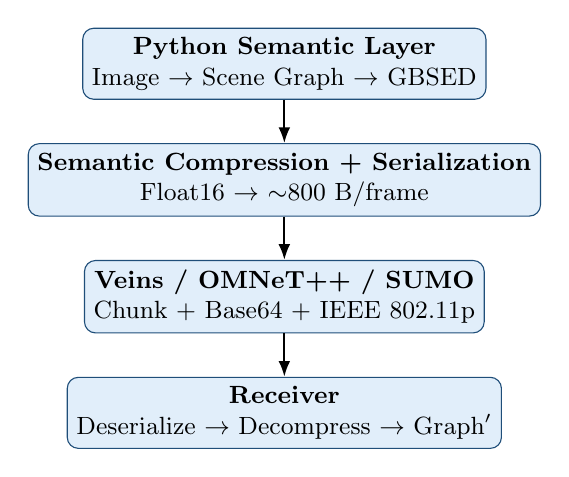
\begin{tikzpicture}[
    box/.style={
        draw=mainblue,
        rounded corners,
        fill=lightblue,
        minimum width=4.7cm,
        minimum height=0.72cm,
        align=center,
        font=\small
    },
    arr/.style={
        -{Latex[length=2mm]},
        thick
    }
]

\node[box] (semantic) {
    \textbf{Python Semantic Layer}\\
    Image $\rightarrow$ Scene Graph $\rightarrow$ GBSED
};

\node[box, below=0.55cm of semantic] (compress) {
    \textbf{Semantic Compression + Serialization}\\
    Float16 $\rightarrow$ $\sim$800 B/frame
};

\node[box, below=0.55cm of compress] (network) {
    \textbf{Veins / OMNeT++ / SUMO}\\
    Chunk + Base64 + IEEE 802.11p
};

\node[box, below=0.55cm of network] (receiver) {
    \textbf{Receiver}\\
    Deserialize $\rightarrow$ Decompress $\rightarrow$ Graph$'$
};

\draw[arr] (semantic) -- (compress);
\draw[arr] (compress) -- (network);
\draw[arr] (network) -- (receiver);

\end{tikzpicture}

\end{center}

\end{frame}


% ============================================================
% SLIDE 13 — EXPERIMENTAL SETUP
% ============================================================
\begin{frame}{Experimental Setup}

\begin{columns}[T]

\column{0.48\textwidth}

\textbf{Vehicular Network}

\begin{itemize}
    \item OMNeT++ + Veins
    \item SUMO mobility
    \item IEEE 802.11p
    \item V2V broadcast
    \item Vehicles move apart
\end{itemize}

\column{0.48\textwidth}

\textbf{Channel Conditions}

\begin{itemize}
    \item Five noise floors
    \item $-98$ to $-80$ dBm
    \item Two driving sequences
    \item Per-chunk TX/RX logs
    \item Distance recorded per packet
\end{itemize}

\end{columns}

\vspace{0.3cm}

\begin{block}{Dataset}
Sequence 1: 20 frames
\hspace{5cm}
Sequence 2: 23 frames
\end{block}

\vspace{0.15cm}

\begin{center}
\scriptsize
Vehicles diverge at right angles at 8 m/s to create increasing separation.
\end{center}

\end{frame}


% ============================================================
% SLIDE 14 — DELIVERY RESULTS
% ============================================================
\begin{frame}{Results: Network Delivery}

\begin{center}

\includegraphics[width=0.57\textwidth]{figures/network_delivery.png}
\end{center}

\vspace{-0.1cm}

{\small
\begin{itemize}
    \item Rising noise and increasing separation sharply reduce payload delivery.
    \item \textbf{Every successfully delivered frame reconstructed exactly.}
    \item Degradation is therefore \textbf{frame availability}, not partial corruption.
   % \item Measured range cliff: approximately \textbf{488 m}.
\end{itemize}
}

\end{frame}


% ============================================================
% SLIDE 15 — FIXED BUDGET, REAL CHANNEL (REDESIGNED)
% ============================================================
\begin{frame}{Results: Same Byte Budget, Real Channel}

\begin{center}

\includegraphics[height=0.82\textheight]{figures/matched_budget.png}
\end{center}

\end{frame}


% ============================================================
% SLIDE 16 — BANDWIDTH COMPARISON
% ============================================================
\begin{frame}{Results: How Much Bandwidth Do Images Need?}

\begin{center}

\includegraphics[width=0.6\textwidth]{figures/bandwidth_gap.png}
\end{center}

\vspace{-0.05cm}
{\small
\begin{itemize}
    \item GBSED preserves \textbf{44/44} safety-critical relations at only
          \textbf{811 B/frame}.
    \item WebP first matches GBSED at \textbf{77,809 B/frame} --- about
          \textbf{96$\times$ more bandwidth}; JPEG does not match within the sweep.
    \item Efficiency: GBSED \textbf{369 B} vs.\ WebP \textbf{35,368 B} per
          preserved safety relation.
\end{itemize}
}

\end{frame}


% ============================================================
% SLIDE 17 — FULL FRAME FEASIBILITY
% ============================================================
\begin{frame}{Results: Full-Frame Transmission Is Infeasible}

\begin{columns}[c]

\column{0.56\textwidth}

\includegraphics[width=\textwidth]{figures/payload_size.png}

\column{0.42\textwidth}
\begin{itemize}
    \item Full JPEG: \textbf{24.8 MB} for 20 frames (\textbf{1531$\times$}).
    \item Transmission time: \textbf{62,118 s} vs.\ a \textbf{125 s}
          vehicle lifetime.
    \item Frames delivered: \textbf{0/20}.
    \item Only \textbf{1.24\%} of the first frame arrived before the
          communication opportunity ended.
\end{itemize}

\vspace{0.2cm}

{\footnotesize \textit{The full image cannot finish transmission within
the vehicle encounter.}}

\end{columns}

\end{frame}


% ============================================================
% SLIDE 18 — GRACEFUL DEGRADATION
% ============================================================
\begin{frame}{Results: Graceful Semantic Degradation}

\begin{center}

\includegraphics[width=0.65\textwidth]{figures/loss_resilience.png}
\end{center}

\vspace{-0.05cm}

\begin{center}
\tiny
The payload packs whole relation slices into independent chunks,
\textbf{safety-critical relations first}. A lost chunk removes a relation
\emph{type} instead of the whole frame.
\end{center}

\end{frame}


\begin{frame}{Why Does Semantic Communication Work Here?}

\noindent
\begin{center}
\textbf{\large Why GBSED fits this task}
\end{center}

\begin{center}
\textbf{The task does not need the whole image.}
\end{center}

\vspace{0.25cm}

\begin{columns}[T]

\column{0.32\textwidth}
\small
\textbf{ 1. Compress the Right Information}

\begin{itemize}
    \item Image has unnecessary visual detail.
    \item GBSED keeps:
    \begin{itemize}
        \item Objects
        \item Positions
        \item Relations
    \end{itemize}
\end{itemize}


\column{0.32\textwidth}
\small
\textbf{ 2. Degrade Differently}

\begin{itemize}
    \item Image compression loses visual detail.
    \item Semantic data loses relation types.
    \item Remaining structure stays meaningful.
\end{itemize}


\column{0.32\textwidth}
\small
\textbf{ 3. Meaning Is Discrete}

\begin{itemize}
    \item Relations: present / absent.
    \item Labels: small integers.
    \item Semantic content can remain exact.
\end{itemize}

\end{columns}
\end{frame}




% ============================================================
% SLIDE 20 — CHALLENGES
% ============================================================
\begin{frame}{Challenges During Implementation}

\small

\begin{itemize}

    \item \textbf{Integrating GBSED with Veins + SUMO}
    \begin{itemize}
        \item Connecting the GBSED encoder--decoder pipeline
        with the Veins wireless network.
        \item Building a GBSED-specific vehicular network scenario.
    \end{itemize}

    \vspace{0.08cm}

    \item \textbf{Adapting Legacy Components}
    \begin{itemize}
        \item RoadScene2Vec (used for \textbf{scene-graph generation})
        relied on an older software stack.
        \item Adapting and consolidating it for our project
        required modifying the existing pipeline.
    \end{itemize}

    \vspace{0.08cm}

    \item \textbf{Risk Assessment Limitations}
    \begin{itemize}
        \item The available risk-assessment images contained only
        one class: \textbf{risky}.
        \item Without a non-risky class, meaningful risk-prediction
        evaluation was not possible.
        \item The whole $\sim$55.4~GB dataset also exceeded our practical
        processing capacity within the available time and CPU resources.
    \end{itemize}

\end{itemize}

\end{frame}

% ============================================================
% SLIDE 21 — LIMITATIONS
% ============================================================
\begin{frame}{Limitations}

\small

\begin{itemize}

    \item \textbf{Risk assessment could not be fully evaluated}
    \begin{itemize}
        \item The available risk-assessment data contained only the
        \textbf{risky} class, with no safe/non-risky cases for comparison.
        \item The original $\sim$55.4~GB dataset was not feasible to
        process with our available time and CPU resources.
    \end{itemize}

    \vspace{0.12cm}

    \item \textbf{Simple network scenario}
    \begin{itemize}
        \item We used only a simple mobility scenario
        to isolate and study the communication behaviour.
        \item Larger and more congested scenarios were not evaluated yet.
    \end{itemize}

    \vspace{0.12cm}

    \item \textbf{Ground-truth limitation}
    \begin{itemize}
        \item We generated our own ground truth for predictions using simple rule-based labels because the original dataset could not
        be processed.
    \end{itemize}

\end{itemize}

\end{frame}
% ============================================================
% SLIDE 22 — CONCLUSION
% ============================================================
\begin{frame}{Conclusion}

\small

\begin{center}
\textbf{What We Demonstrated}
\end{center}

\vspace{0.1cm}

\begin{itemize}

    \item Integrated the GBSED pre-trained encoder--decoder with
          \textbf{Veins, OMNeT++, SUMO}
          for vehicular communication.

    \vspace{0.1cm}

    \item Successfully reconstructed the semantic scene graph
          when network frames were delivered.

    \vspace{0.1cm}

    \item At the \textbf{same byte budget}, GBSED preserved
          safety-critical relations, while JPEG/WebP did not.

    \vspace{0.1cm}

    \item WebP required approximately \textbf{96$\times$ more bandwidth}
          to achieve the same safety-relation preservation.

    \vspace{0.1cm}

    \item Demonstrated \textbf{graceful semantic degradation}:
          a lost chunk can remove a relation type rather than
          destroying the entire frame.

\end{itemize}

\end{frame}

% ============================================================
% SLIDE 23 — FUTURE WORK
% ===========================================================
\begin{frame}{Future Work}

\small

\begin{itemize}

\item \textbf{Expand the vehicular network scenario}
\begin{itemize}
    \item Introduce more vehicles, realistic mobility, wireless
    contention, and varied network configurations.
\end{itemize}

\item \textbf{Complete the risk assessment pipeline}
\begin{itemize}
    \item Evaluate risk prediction using more diverse and properly
    labelled driving scenarios.
\end{itemize}

\item \textbf{Connect risk assessment to vehicle actions}
\begin{itemize}
    \item Use predicted risk to drive appropriate vehicle responses
    through a \textbf{control-in-the-loop} framework.
\end{itemize}

\item \textbf{Study semantic information requirements}
\begin{itemize}
    \item Investigate how much semantic information is needed for
    reliable risk assessment and decision-making.
\end{itemize}

\end{itemize}

\end{frame}


\begin{frame}{Individual Contributions}

\small

\begin{columns}[T]

\begin{column}{0.32\textwidth}

\begin{center}
\textbf{Maisha Sanjida}
\end{center}

\begin{itemize}
\item Veins + SUMO simulation setup and necessary Simulation file creation
\item Binary payload serialization \& network transmission
\item Risk assessment \& ground-truth generation
\end{itemize}

\end{column}

\begin{column}{0.32\textwidth}

\begin{center}
\textbf{Saeera Tanjim}
\end{center}

\begin{itemize}
\item Different Simulation scenario configurations
\item GBSED encoder--decoder evaluation
\item Packet delivery and range analysis from results
\end{itemize}

\end{column}

\begin{column}{0.32\textwidth}

\begin{center}
\textbf{Mahdi Islam}
\end{center}

\begin{itemize}
\item Encoder--decoder integration in Veins
\item Payload encoding, chunking \& decoding
\item Graceful degradation \& performance analysis between JPEG, WebP and semantic scene graph
\end{itemize}

\end{column}

\end{columns}

\end{frame}



\begin{frame}{GitHub \& Resources}

\begin{center}

\textbf{\large Original GBSED Repository}

\vspace{0.08cm}

\href{https://github.com/philpolo/gbsed}
{\small \texttt{github.com/philpolo/gbsed}}

\vspace{0.4cm}

\textbf{\large Our GBSED Repository}

\vspace{0.08cm}

\href{https://github.com/sahil0319/gbsed}
{\small \texttt{github.com/sahil0319/gbsed}}

\vspace{0.4cm}

\textbf{\large Our Veins Repository}

\vspace{0.08cm}

\href{https://github.com/Loona6/gbsed_veins}
{\small \texttt{github.com/Loona6/gbsed\_veins}}

\end{center}

\vfill

\begin{center}
\small
All implementation, simulation, and supporting code are available in the repositories above.
\end{center}

\end{frame}







% ============================================================
% SLIDE 25 — REFERENCES
% ============================================================
\begin{frame}{References}

\scriptsize

\nocite{malawade2022roadscene2vec}

\bibliographystyle{IEEEtran}
\bibliography{ref}

\end{frame}
% ============================================================
% FINAL SLIDE
% ============================================================
\begin{frame}

\begin{center}

\vspace{1.5cm}

{\Huge \textbf{Thank You}}

\vspace{0.5cm}

{\Large Any Questions?}

\vspace{0.8cm}


\end{center}

\end{frame}


\end{document}
